\section{Instances}\label{sec:instances}
To assess our methods on realistic instances of the problem, we use the actual wind-optimal trajectories for transatlantic flights on July 29, 2012, as was done in previous work~\cite{rodionova16}.
In these trajectories, each flight has a constant (cruising) altitude 
and constant speed, to within (classical) machine precision,
though our methods generalize to instances without these special properties.

One perspective into the nature of an instance of the deconflicting problem is the \emph{conflict graph}, whose vertices correspond to flights and which has an edge between a pair of vertices if there is at least one potential conflict between the corresponding flights.
Note that the conflict graph for a given set of trajectories depends on the parameters of the problem.
In the case of only departure delays, whether or not a potential conflict, and thus an edge in the conflict graph, exists between two flights is a function of $d_{\max}$.
For a certain value of $d_{\max}$, the conflict graph may contain several connected components, which can be considered as smaller, independent instances.
Figure~\ref{fig:num-CCs-vs-dmax} shows this dependence of the number of connected components on the maximum delay $d_{\max}$,
and Figure~\ref{fig:hist-CC-sizes} shows the distribution of the sizes of the connected components for various values of $d_{\max}$.
Interestingly, 
most of the connected components are very small; for example, with $d_{\max}= 60$ minutes, approximately $75\%$ of the connected components contain no more than $10$ flights.

\begin{figure*}[p]
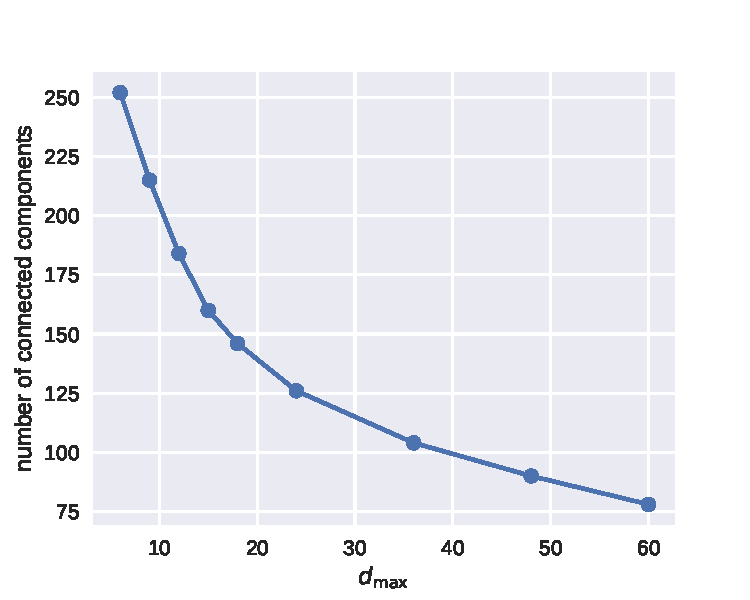
\includegraphics[width=\columnwidth]{pics/instances/num_cc.pdf}
\caption[Number of connected components vs. $d_{\max}$]{Number of connected components versus $d_{\max}$.}
\label{fig:num-CCs-vs-dmax}
\end{figure*}

\begin{figure*}[p]
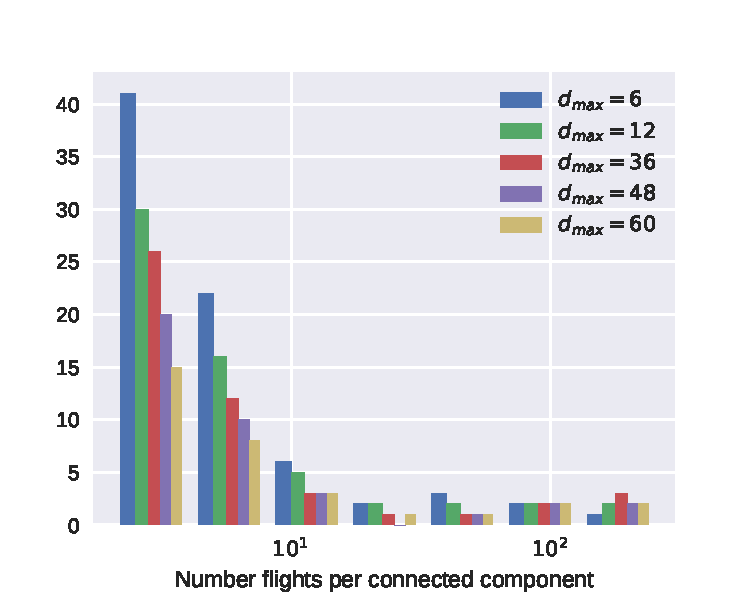
\includegraphics[width=\columnwidth]{pics/instances/analysis_cc.pdf}
\caption[Histogram of connected component sizes]{Histogram of the number of flights per connected component, regardless the maximum delay time.}
\label{fig:hist-CC-sizes}
\end{figure*}

As part of our analysis, we also studied the probability
distribution of the connectivity, namely the number of flights
for which a given flight share a potential conflict with. 
Figure~(\ref{fig:hist-degree}) shows
the distribution of degrees in the conflict graph for $d_{\max}=60$,
which seem to be approximately distributed according to a power law, i.e. 
the number of vertices with degree $d$ is proportional to $d^{\alpha}$.
This is consistent with a so-called ``small-world'' model believed to be typical of many real-world graphs~\cite{barabasi:99}, which are generated by preferential attachment and resultingly contain a few number of highly-connected hubs, as is the case with air traffic.
Figure~(\ref{fig:exponent-vs-dmax}) shows the dependence of this empiral power-law exponent $\alpha$ as a function of $d_{\max}$.
As $d_{\max}$ increases, the exponent decreases.
The larger the delay, the less the structure of the trajectories matters and the flatter the distribution of degrees in the conflict graph.

\begin{figure*}[p]
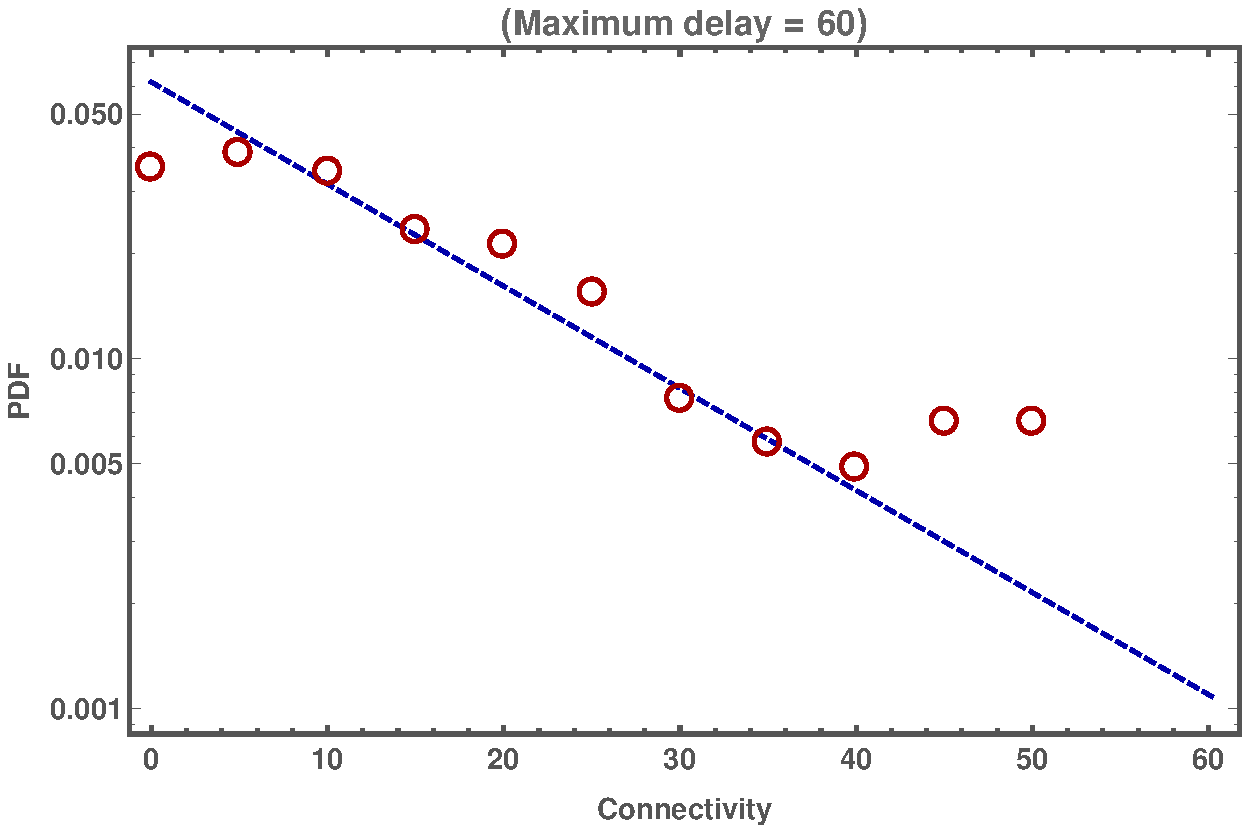
\includegraphics[width=0.95\columnwidth]{pics/instances/connectivity_pdf.pdf}
\caption[Histogram of degrees]{Histogram of the degrees of vertices in the conflict graph for $d_{\max} = 60$. 
The distribution of the degrees approximately follows a power law, with the exponent depending on $d_{\max}$.
}
\label{fig:hist-degree}
\end{figure*}

\begin{figure*}
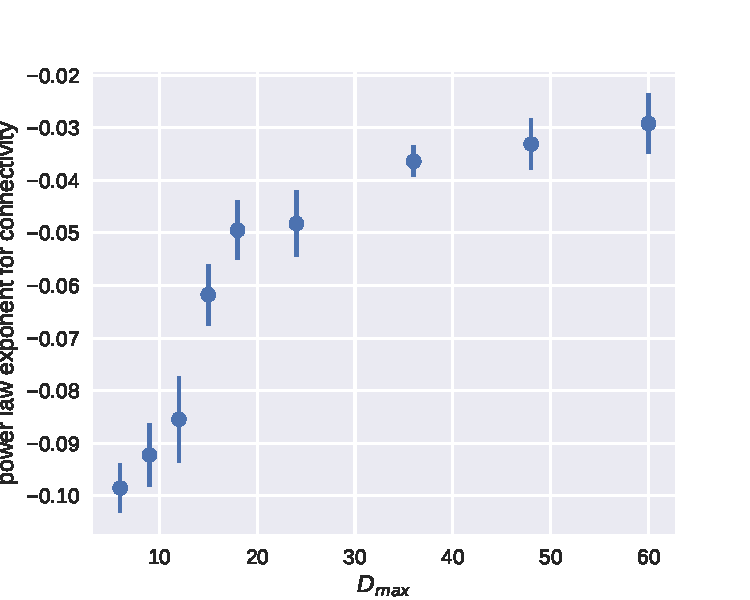
\includegraphics[width=0.95\columnwidth]{pics/instances/connectivity_pl.pdf}
\caption[Power-law exponent vs. $d_{\max}$]{Empirical power-law exponent versus $d_{\max}$.}
\label{fig:exponent-vs-dmax}
\end{figure*}

In many cases, generally hard problems are easy when restricted to tree-like instances~\cite{bertele1972, halin1976s}.
For example, if the conflict graph here is a tree, then the optimum could be easily found by propogating the delays along the tree;
on the other hand, if the conflict graph is a complete graph, finding the optimum is much harder.
The tree-width of a graph formalizes this notion of tree-likeness, ranging from $1$ for a tree to $n-1$ for fully connected graph.
We examine the treewidth of the connected components as a proxy for the hardness of the instances they represent.
Figure~\ref{fig:hist-tws} shows that most connected components are very tree-like, while there are a few strongly-connected components.

\begin{figure}
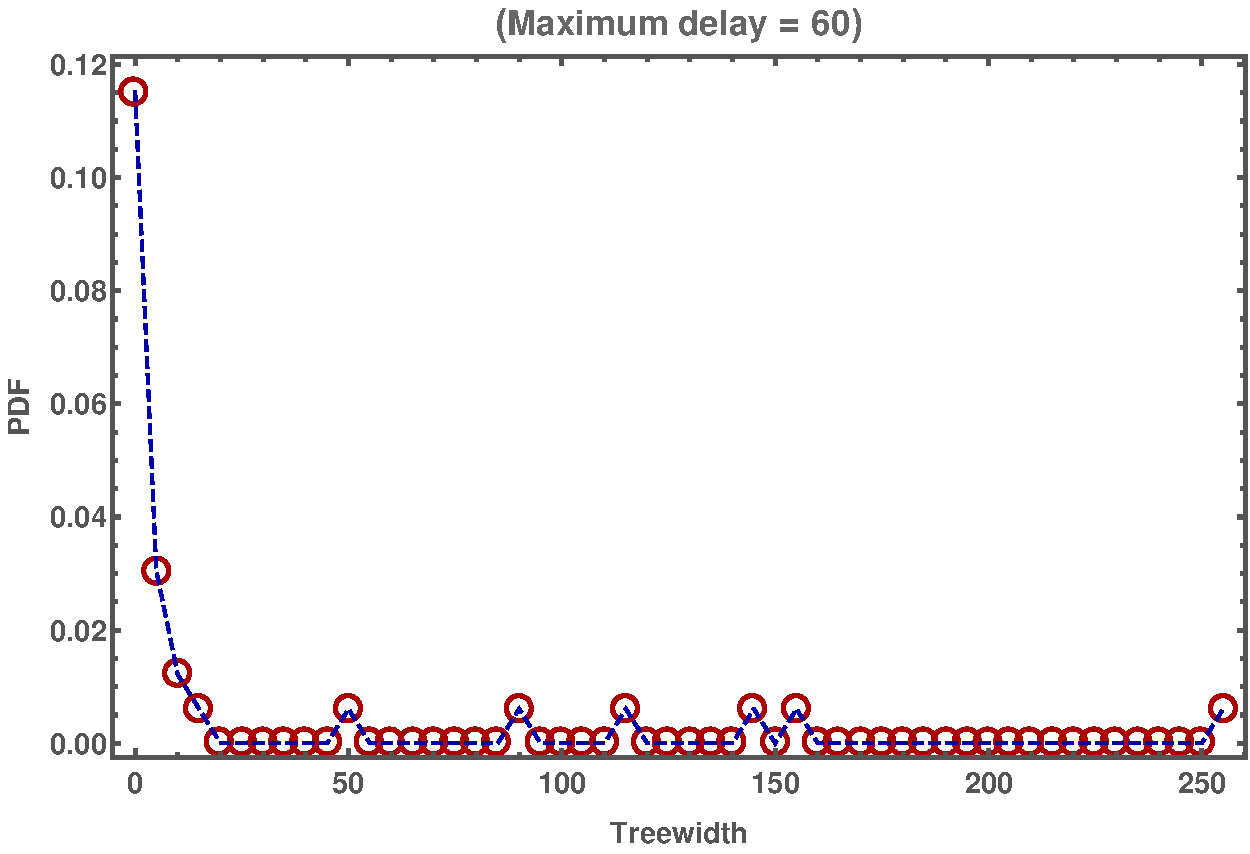
\includegraphics[width=\columnwidth]{pics/instances/treewidth_histogram.pdf}
\caption[Histogram of connected component treewidths]{Histogram of the treewidths of the connected components of the conflict graph for various values of $d_{\max}$.}
\label{fig:hist-tws}
\end{figure}

Figure~\ref{fig:tw-vs-CC-size} shows that the treewidth of a connected component scales approximately linearly with its size.
This indicates that realistic instances of the deconflicting are indeed hard, and not restricted to easier (bounded tree-width) instances of the generally hard problem.
Moreover, the correlation $\gamma$ between the tree-width of a connected component and its size increases with $d_{\max}$, as shown in Figure~\ref{fig:treewidth-size-correlation}.
The larger $d_{\max}$, the more potential conflicts there are;
restricting $d_{\max}$ also restricts the number of conflicts.

\begin{figure*}
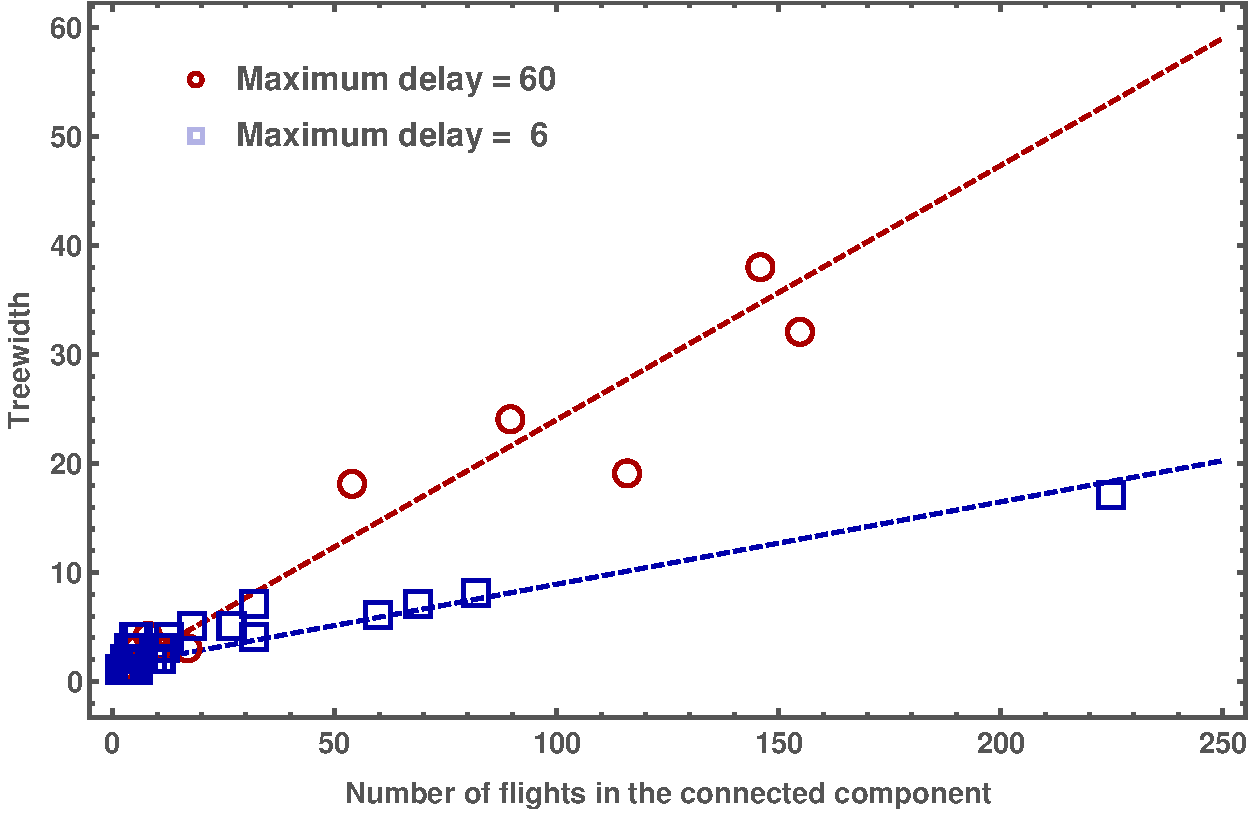
\includegraphics[width=\columnwidth]{pics/instances/treewidth_connectivity.pdf}
\caption[Correlation between connected component size and treewidth]{
The treewidths of connected components versus their sizes for various values of $d_{\max}$.
The correlation is approximately linear, with a slope $\gamma$ that depends on $d_{\max}$.
}
\label{fig:tw-vs-CC-size}
\end{figure*}

\begin{figure*}
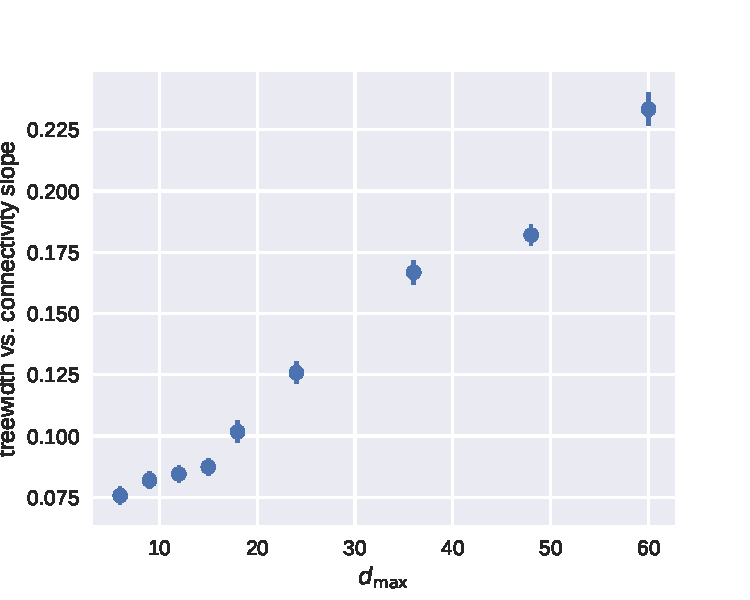
\includegraphics[width=\columnwidth]{pics/instances/treewidth_pl.pdf}
\caption[Treewidth-size correlation coefficient vs. $d_{\max}$]{Slope $\gamma$ as a function
  of the maximum delay time.}
\label{fig:treewidth-size-correlation}
\end{figure*}
